\documentclass[12pt]{article}

\usepackage{sbc-template}
\usepackage{graphicx,url}
\usepackage{algorithm}
\usepackage{algpseudocode}
\usepackage{amsmath,amssymb,exscale}
\usepackage[brazil]{babel}

\usepackage{xcolor}
% Definindo novas cores
\definecolor{verde}{rgb}{0,0.5,0}
% Configurando layout para mostrar codigos C++
\usepackage{listings}
\lstset{
  language=C++,
  basicstyle=\ttfamily\small,
  keywordstyle=\color{blue},
  stringstyle=\color{verde},
  commentstyle=\color{red},
  extendedchars=true,
  showspaces=false,
  showstringspaces=false,
  numbers=left,
  numberstyle=\tiny,
  breaklines=true,
  backgroundcolor=\color{green!10},
  breakautoindent=true,
  captionpos=b,
  xleftmargin=0pt,
}

\usepackage[utf8]{inputenc}

\sloppy

\title{AA de Grafos e Algoritmos \\ Algoritmo de Kruskal}

\author{ Jamile Santos\inst{1}, Liliane Neves\inst{1}, Victor Pedro\inst{1} }

\address{
	Departamento de Ciência da Computação -- Instituto Multidisciplinar \\ Universidade Federal Rural do Rio de Janeiro (UFRRJ)
	\email{milysantos18@gmail.com,lilianeneves8@gmail.com, victorp@r7.com}
}

\begin{document}
	\maketitle
 \nocite{*} 
\begin{abstract}
	This paper describes the study about how to implement an algorithm capable of divide a valued graph $G=(V,E)$ in $k$-groups of vertices in a way that the weight of the sum of the edges is the smallest possible. To solve this problem, the algorithm have to find a minimum spawning tree in the graph and after that eliminate the $k-1$ edges. To find the minimum spawning tree will be used the Kruskal's algorithm.
\end{abstract}

\begin{resumo}
	Este relatório descreve o estudo sobre como implementar um algoritmo capaz de separar um grafo valorado $G=(V,E)$ em $k$-grupos de vértices de forma que a soma do peso das arestas seja a menor possível. Para resolver este problema, o algoritmo deve encontrar uma árvore geradora mínima no grafo e após isso eliminar as $k-1$ arestas. Para encontrar a árvore geradora mínima será utilizado o algoritmo de Kruskal.
\end{resumo}

\section{Introdução}
	Dado um grafo não orientado conectado, uma árvore de dispersão deste grafo é um sub-grafo, que é uma árvore que conecta todos os vértices. 
	
	Um único grafo pode ter diferentes árvores de extensão. Nós podemos assinalar um peso a cada aresta, que é um número que representa quão desfavorável ela é, e atribuir um peso a árvore de extensão calculado pela soma dos pesos das arestas que a compõem.
	
	Uma árvore de extensão mínima (também conhecida como árvore de extensão de peso mínimo ou árvore geradora mínima) é então uma árvore de extensão com peso menor ou igual a cada uma das outras árvores de extensão possíveis. Generalizando, qualquer grafo não direcional (não necessariamente conectado) tem uma floresta de árvores mínimas, que é uma união de árvores de extensão mínimas de cada uma de suas componentes conexas.
	
	Este trabalho objetiva dissertar sobre o uso do algoritmo de Kruskal no desafio de encontrar $k$ árvores a partir do grafo inicial de forma que a soma dos pesos das arestas destes sub-grafos seja a menor possível.
	
\section{Árvore Geradora Mínima}
	Este problema, como muitos semelhantes, tem seu foco em encontrar uma Árvore Geradora Mínima (MST - Minimum Spawning Tree)  para um grafo conhecido.
	
	Há uma solução genérica para este problema, que serve de base para o algoritmo de Kruskal, que é o discutido neste trabalho. Este algoritmo genérico mantém um conjunto de arestas $A$ e a seguinte invariante:
	
	A cada iteração, $A$ é subconjunto de arestas de uma MST. 
	
	O algoritmo mantém esta invariante adicionando ao conjunto $A$, a cada iteração, uma aresta $(u,v)$ de maneira que a união de $A$ com $(u,v)$ seja um subconjunto de uma MST \cite{paulo:15}.
	
	No algoritmos da figura~\ref{fig:gen_mst} temos as seguintes variáveis: $A$ é o vetor auxiliar onde a MST será armazenada, $u$ e $v$ são os vértices que serão ligadas pela menor aresta possível.
	
\begin{figure}[ht]
    \centering
    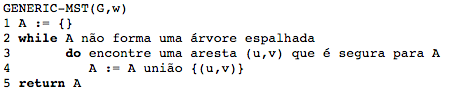
\includegraphics[width=1\textwidth]{imagens/generic_mst.png}
    \caption{Algoritmo MST Genérico}7
    \label{fig:gen_mst}
\end{figure}



\section{O Algoritmo de Kruskal}
O algoritmo de Kruskal propõe que um grafo qualquer seja considerado uma floresta de árvores compostas por apenas um vértice e procura, a cada iteração, conectar duas árvores distintas da floresta através de uma aresta que possua peso mínimo \cite{knuth:84}.

Dessa forma, suponha que, numa determinada iteração, o algoritmo escolher a aresta $(u,v)$ para ser inserida no conjunto $A$ e que a aresta $(u,v)$ conecte a árvore $C_i$ à árvore $C_2$. Observe que, dentre todas as arestas que conectam duas componentes distintas nesta iteração, $(u,v)$ é uma das que possui menor peso, pois foi escolhida. Logo, nesta iteração, para qualquer corte que separe $u$ de $v$, $(u,v)$ é uma aresta leve pelo fato de não existir aresta de menor peso separando duas componentes nesta iteração \cite{knuth:84}.

\begin{figure}[ht]
    \centering
    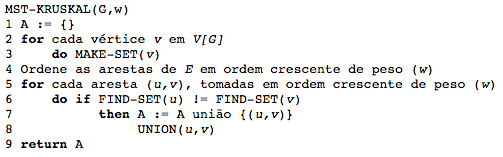
\includegraphics[width=1\textwidth]{imagens/mst_kruskal.png}
    \caption{Algoritmo MST Kruskal}
    \label{fig:mst_kruskal}
\end{figure}

A Figura~\ref{fig:exec_kruskal} exemplifica uma execução do algoritmo de Kruskal. É possível notar que as arestas são visitadas em ordem crescente de peso e, para que uma aresta seja inserida no conjunto $A$, seus vértices adjacentes devem pertencer a componentes diferentes. Neste pseudocódigo, $V$ representa o conjunto de vértices do grafo $G$, e $u$ e $v$ representam os vértices que serão ligados pela aresta selecionada, e $E$ é o conjunto de arestas do grafo.

\begin{figure}[ht]
    \centering
    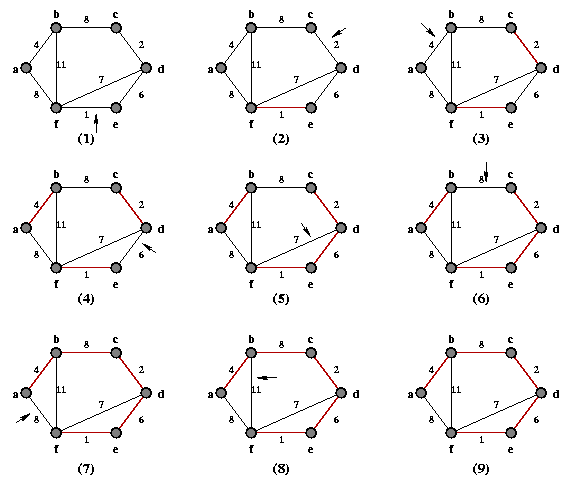
\includegraphics[width=1\textwidth]{imagens/execucao_kruskal.png}
    \caption{Algoritmo MST Genérico}
    \label{fig:exec_kruskal}
\end{figure}


\section{Análise de Complexidade do Algoritmo}
		A complexidade do Algiritmo é: T(N) = $\Theta (E\log E)$, ou $\Theta (E\log V)$. A ordenação das arestas tem tempo $\Theta (E\log E)$. Depois da ordenação, há uma iteração por todas as arestas e é aplicada a união, esta operação é aproximadamente $\Theta (\log V)$. Portanto, a complexidade geral do algoritmo é  $\Theta(E\log E + E\log V)$. O valor de $E$ pode ser no máximo $V^2$, logo, $\Theta(\log V)$ e $\Theta(\log E)$ são as mesmas. Dessa forma podemos afirmar que a complexidade geral do algoritmo é $\Theta (E\log E)$ ou $\Theta (E\log V)$. \cite{geeks:2012}

\section{Conclusões}
Como foi proposto, a implementação é capaz de separar o grafo em árvores conexas pela aresta de menor peso possível, utilizando uma Árvore Geradora Mínima através do algoritmo de Kruskal.

	Os resultados obtidos pelo programa nos testes realizados apresentam sempre resultados corretos e tempos de execução pequenos, mesmo aumentando o número de vértices e arestas.
	

\subsection{Resultados}

O algoritmo foi feito executandocom G++ num MacBook Pro OSX Yosemite core i7, 16GB de RAM e em um MacBook OSX Mavericks, ambos utilizaram o Xcode 7 como IDE C++.

\begin{figure}[ht]
    \centering
    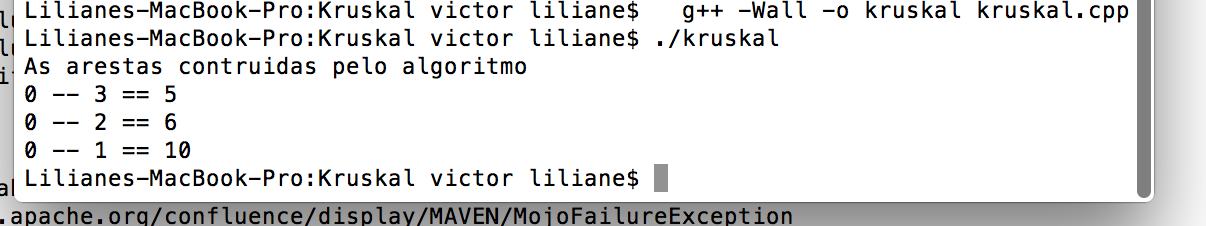
\includegraphics[width=1\textwidth]{imagens/figura1.png}
    \caption{Código executado}
\end{figure}


\bibliographystyle{sbc}
\bibliography{relatorio}


\end{document}


